\documentclass{bioinfo}
\copyrightyear{2009}
\pubyear{2009}

\bibliographystyle{natbib}
\usepackage{subfigure}

% \usepackage{flafter,epsf}       
% \usepackage{amsmath}
% \usepackage{amsfonts,amsbsy,amssymb,bbm}
% \usepackage{amsthm}  %% proof enviroment
% \usepackage{natbib}
% %\usepackage{showkeys}

% \sloppy 
% \usepackage{graphicx}

% \bibliographystyle{mbe_bibliography}

% \input{epsf}

% \newcommand {\rel} {\mathbb{R}}
% \newcommand {\com} {\mathbb{C}}
% \newcommand {\nat} {\mathbb{N}}
% \newcommand {\rat} {\mathbb{Q}}
% \newcommand {\ganz} {\mathbb{Z}}
% \newcommand {\indicator} {\mathbbm{1}}


% \newtheorem{defi}{Definition}
% \newtheorem{theo}{Theorem}
% \newtheorem{corol}{Corollary}
% \newtheorem{prop}{Proposition}
% \newtheorem{example}{Example}
% \newtheorem{lemma}{Lemma}
% \newtheorem{problem}{Problem}[section]

% \textheight 21cm
% \textwidth 16cm
% \oddsidemargin -0.1cm
% \evensidemargin -0.1cm

\newlabel{d2_section}{A}
\newlabel{mst_section}{B}
\newlabel{sim_results}{C}
\newlabel{real_results}{D}
\newlabel{ESTsim_sup}{C.1}
\newlabel{seq_time}{S4}

\begin{document}

\firstpage{1}

\title[PEACE cluster]{PEACE: {\underline P}arallel {\underline E}ST {\underline A}nalysis
  and {\underline C}lustering {\underline E}ngine}
\author{D.M. Rao\,$^{1}$, J.C. Moler\,$^{1}$, M. Ozden\,$^1$, Y. Zhang\,$^{1}$,
  C. Liang$^{1,2*}$\, and J.E. Karro\,$^{1,3}$\footnote{to whom
    correspondence should be addressed}}
\address{$^1$ Department of Computer Science and Software Engineering, \\
  $^2$ Department of Botany, \\
  $^3$ and Department of Microbiology, Miami University, Oxford, Ohio,
  USA}

\history{Received on XXXXX}

\editor{Associate Editor: XXXXX}

\maketitle

\begin{abstract} 
  \noindent {\bf Summary: } \textsc{peace} is a software tool for the
  clustering of large sets of Expressed Sequence Tags by gene
  association, executable as a single processor tool with the
  infrastructure for distributing its computation over multiple
  processors on any platform supporting {\bf MPI}.  \textsc{peace}
  demonstrates considerably higher sensitivity, than other tools
  addressing the EST clustering problem, while exhibiting slightly
  faster performance.\\
  {\bf Availability: } Source Code and manual are available at
  www.conifergdb\\.org/PEACE.php.  Code is implemented in C++, and ready
  to run as a command line tool under Windows, Linux and OS X. \\
  {\bf Contact: } karroje@muohio.edu \\
  {\bf Supplementary Information:} A supplementary materials section
  has been submitted with this paper that contains additional details on the
  algorithm and additional results.
\end{abstract}


\section {Introduction}

Expressed Sequence Tags, or ESTs, are short DNA sequences obtained
from cDNA that represent transcripts of expressed genes.  They have
proved a powerful tool in the study of genes and gene organization, helping us to
identify genes and providing us access to the
transcriptome.  They are an inexpensive and easy way to obtain DNA-level
knowledge about any genome, but the computational cost of the EST analysis
is high [\cite{Nagaraj07}].

A critical step in the analysis of any EST data set is that of
clustering: partitioning the data into disjoint sets based on gene
association.  Clustering is generally done through overlap
identification, but the accuracy of alignments can be disrupted by EST
sequencing error.  Single base read errors are reported to occur in as
much as 5\% of bases [\cite{Nagaraj07}], while insertions, deletions and stuttering can
also be an issue; the genetic variations inherent in a set of transcriptomes 
can also disrupt overlap-based detection.  Further, the large size of
EST data sets poses its own problems; computing alignments of all
pairs is infeasible in terms of both runtime and memory usage.

Here we present \textsc{peace}, a tool for the clustering of EST sets
by gene, applicable to ESTs of length 150 bp or greater using the
default parameters.  Using a {\it minimum spanning tree} (MST) based
clustering strategy [\cite{Jain99,Wan08}] and the $d^2$ sequence
distance function [\cite{Hide94}], \textsc{peace} generates
the MSTs using a tailored version of Prim's algorithm [\cite{Prim57}].
The result is a clustering tool that is considerably more sensitive to
sequencing errors than the competing \textsc{wcd} tool
[\cite{Hazelhurst08a}] and others in the literature without any
sacrifice of performance (e.g. [\cite{Burke99}, \cite{Slater00},
\cite{Huang99}, \cite{Parkinson02}, \cite{Kalyanaraman03},
\cite{Malde03}, \cite{Ptitsyn05}, \cite{Picardi09}]).

\section {Methods}

The clustering performed by \textsc{peace} is based on the use of minimum
spanning trees (MSTs), known to be an effective approach for narrow
band single linkage clustering [\cite{Jain99,Wan08}]. We use the $d^2$
distance measure [\cite{Hide94}] to represent edge weights.  Prim's
algorithm [\cite{Prim57}] then allows us to efficiently calculate an
MST from which we can infer a high-quality clustering solution.

The $d^2$ distance measure used to assign edge weights is an
alignment-free measurement of sequence distance calculated
significantly faster than a alignment \cite{Hide94,Foret09}.  $d^2$
works by comparing the frequency of words (strings of a fixed length)
appearing in a limited region of each string.  ESTs overlapping by a
sufficient length will share neighborhoods of enough similarity to
ensure a small distance even in the presence of a moderate number of
base errors.  Our method of calculating $d^2$, the {\it two-pass $d^2$
  heuristic}, is a refinement of that used in the \textsc{wcd}
clustering tool [\cite{Hazelhurst08a}].  We augment the computation
with a preliminary pass that narrows down the two regions of maximum
similarity, and then explore those local regions in more detail.

We can model the EST input as a weighted, undirected graph: the ESTs
are represented as nodes, with $d^2$ sequence distances assigned to
the connecting edges as weights.  Conceptually, we want to remove each
edge exceeding a threshold score from the complete graph, and define
our partitions by the remaining connected components of the graph.  An
edge with a large weight connects ESTs which are likely unrelated;
once such edges are removed, the components define a series of
overlaps.  Hence those ESTs that can still be connected by some path
correspond to the same gene.  However, such an approach requires the
calculation of all edge weights, a task infeasible both in terms of
runtime and memory usage for the data set sizes we expect to process.

We approach the problem by generating a minimum spanning tree of the
described graph, then removing edges exceeding our threshold.  By
using Prim's algorithm we are able to calculate edge weights
on-the-fly (reducing memory requirements), and we can skip the
calculation of a majority of edge distances using the $u/v$ and $t/v$
filtering heuristics employed in \textsc{wcd} [\cite{Hazelhurst08a}].
These heuristics allow us to quickly dismiss many of the edges as too
large without the need to apply the full $d^2$ algorithm (see
Sections~\ref{d2_section} and \ref{mst_section} of the Supplementary
Materials for more details). 

\section{Results}

We have tested \textsc{peace} on both simulated and real data,
comparing results against those produced by the \textsc{wcd}
clustering tool [\cite{Hazelhurst08a}] and the \textsc{cap3} assembly
tool [\cite{Huang99}] (which calculates a cluster as an intermediate
step).  For our simulation tests we used the {\bf ESTSim} tool
[\cite{Hazelhurst03}] to generate simulated ESTs under varying models
of error (Supplementary Materials, Section~\ref{ESTsim_sup}),
generating the fragments from the list of 100 zebra fish genes used in
the \textsc{wcd} testing [\cite{Hazelhurst08a}].  Tool parameters were
taken to match, as closely as possible, those used in the \textsc{wcd}
study (see supplementary materials).  Our primary methods of quality
assessment were {\it sensitivity} (the fraction of EST pairs from the
same gene that were correctly clustered together) and {\it Type 1
  error} (the fraction of genes that were divided between clusters)
[\cite{Wang04,Hazelhurst08a}]; other measurements are also discussed
in the supplementary materials.  In Figure~1 (left) we see a
significant improvement of \textsc{peace} (blue) over \textsc{wcd}
(green) and \textsc{cap3} (black) in its sensitivity to sequencing
errors, while in Figure~1 (right) we see a comparable
improvement in Type 1 error.  In Figure~2 we look at
the number of singleton clusters (ESTs not joined to any cluster),
which will not occur in our simulated sets; we again see significant
improvement in \textsc{peace}.  The sequential runtime of
\textsc{peace} is slightly improved over that of \textsc{wcd} (see
Supplementary Materials, Figure~S4).

\begin{figure*}[b]
\centerline{
\includegraphics[scale=0.5]{SeT1.eps} 
}
\label{SeT1}
\caption{Comparisons of Sensitivity and Type 1 error, based on the
  average over 30 Simulated EST sets derived from 100 zebra fish genes
  (see Supplementary Materials, Section~\ref{sim_results}, for more
  details).   Blue/Solid = \textsc{peace}, Green/Dash =
  \textsc{wcd}, Black/Dot-Dash = \textsc{cap3}; vertical tics = 95\% confidence
  intervals on estimates.  Intervals are not presented for Type 1
  error due to the extremely small variance.}
\end{figure*}

\begin{figure*}[b]
\centerline{
\includegraphics[scale=0.35]{singletons.eps}
}
\label{singletons}
\caption{Average number of ESTs flagged as singletons by each tool
  when run on the simulated sequences; correct answer in all cases is
  zero.  Blue/Solid = \textsc{peace}, Green/Dash = \textsc{wcd},
  Black/Dot-Dash = \textsc{cap3}.}
\end{figure*}

In applying the tools to real data, we started with a set of
approximately $190,000$ ESTs derived from the {\it Chlamydomonas
  reinhardtii} genome.  To compute sensitivity we used the {\it gmap}
tool [\cite{Wu05}] to map the EST set to the genome, taking this as
our reference clustering.  We see slight improvements in
\textsc{peace} over \textsc{wcd} in both sensitivity and Type 1 error
(both significantly out preforming \textsc{cap3}).  Using the mouse EST
set used in Hazelhurst {\it et al.}  [\cite{Hazelhurst08a}]
\textsc{peace} again shows slight improvements in sensitivity and Type
1 error rates, with an 18\% speed up for \textsc{peace} (see
Supplementary Materials, Section~\ref{real_results}, for more
details).

\section{Acknowledgements}

Dr. Karro was funded under a PhRMA Foundation Informatics Research
Starters Grant while conducting this research.  We would also like to
acknowledge Iddo Friedberg, David Woods, Jens Mueller and David
Scoville at Miami University for their help with this project.

\vspace{3mm}
%Bib TeX

\bibliography{peace.bib}



\end{document}


% LocalWords:  arallel nalysis lustering ngine Rao Moler Ozden Zhang Liang ESTs
% LocalWords:  Karro XXXXX transcriptome pre isoforms SNPs unsequenced runtime
% LocalWords:  chlamydomondomonas ESTate PaCE xsact CLU WCD Hazelhurst et al th
% LocalWords:  CHUN nalyzer Prim's MSTs subgraph MPI SourceCode ESTSim runtimes
% LocalWords:  ests Chlamydomonas Reihartdii gmap CDNA transcriptomes cDNA www
% LocalWords:  reinhartdii conifergdb DNAc bp wcd reinhardtii PhRMA Iddo
% LocalWords:  Friedberg Scoville
